    \section{Low-Voltage Induced Random Bit Errors in Quantized DNN Weights}
\label{sec:supp-main}

We provide a more detailed discussion of the considered error model: random bit errors, induced through low-voltage operation of memories commonly used on DNN accelerators \cite{KimDATE2018,KoppulaMICRO2019}. Work such as \cite{ChandramoorthyHPCA2019,KoppulaMICRO2019} model the effect of low-voltage induced bit errors using two parameters: the probability $\pfault$ of bit cells in accelerator memory being faulty at a given low voltage and the probability $\perror$ that a faulty bit cell results in a bit error on access.
Following measurements in works such as \cite{GanapathyHPCA2019,KimDATE2018}, we assume that these errors are \emph{not} transient errors by setting $\perror = 100\%$ such that the overall probability of bit errors is $p := \pfault \cdot \perror = \pfault$. In doing so, we consider the worst-case where faulty bit cells \emph{always} induce bit errors. However, the noise model from the main paper remains valid for any arbitrary but fixed $\perror \neq 100\%$. For the reminder of this document, we assume the probability of bit error $p = \pfault$, with $\perror = 100\%$, as in the main paper. In the following section, we describe the two parameters, $\pfault$ and $\perror$, in more details.

\begin{table}[t]
	\centering
	\caption{\textbf{Quantization-Aware Training Accuracies.} Clean \TE for $m = 8$ bits or lower using our robust fixed-point quantization. We obtain competitive performance for $m = 8$ and $m = 4$ bits. On \CifarH, a Wide ResNet (WRN) clearly outperforms our standard SimpleNet model. Batch normalization (BN), improving \TE slightly on \CifarT, is significantly less robust than group normalization (GN), \cf \tabref{tab:supp-bn}. * For $m \leq 4$, we report results with weight clipping, \Clipping[$0.1$].}
	\label{tab:supp-accuracy}
	\vspace*{-0.25cm}
	\hspace*{-0.25cm}
	\begin{subfigure}[t]{0.19\textwidth}
		\vspace*{0px}
		\small
		\begin{tabular}{|@{\hskip 4px}l@{\hskip 4px}|@{\hskip 4px}c@{\hskip 4px}|}
			\multicolumn{2}{c}{\bfseries \CifarT}\\
			\multicolumn{2}{c}{\bfseries SimpleNet+GN}\\
			\hline
			Quant. $m$ & \TE in \%\\
			\hline
			-- & 4.34\\
			8 & \bfseries 4.32\\
			4* & 5.29\\
			3* & 5.71\\
			\hline
		\end{tabular}
	\end{subfigure}
	\begin{subfigure}[t]{0.28\textwidth}
		\vspace*{0px}
		\small
		\begin{tabular}{|@{\hskip 4px}l@{\hskip 4px}|@{\hskip 4px}c@{\hskip 4px}|@{\hskip 4px}c@{\hskip 4px}|}
			\multicolumn{3}{c}{\bfseries \CifarT}\\
			\multicolumn{3}{c}{\bfseries Arch. Comparison}\\
			\hline
			Model & no Quant. & $m = 8$\\
			\hline
			SimpleNet+GN & 4.34 & 4.32\\
			SimpleBet+BN & 4.04 & 3.83\\
			ResNet-50+GN & 5.88 & 6.81\\
			ResNet-50+BN & \bfseries 3.91 & \bfseries 3.67\\
			\hline
		\end{tabular}
	\end{subfigure}\\[4px]
	
	\hspace*{-0.5cm} 
	\begin{subfigure}[t]{0.19\textwidth}
		\vspace*{0px}
		\small
		\begin{tabular}{| l | c |}
			\multicolumn{2}{c}{\bfseries \MNIST}\\
			\hline
			Quant. $m$ & \TE in \%\\
			\hline
			4 & 0.4\\
			2* & 0.47\\
			\hline
		\end{tabular}
	\end{subfigure}
	\begin{subfigure}[t]{0.2\textwidth}
		\vspace*{0px}
		\small
		\begin{tabular}{| l | c |}
			\multicolumn{2}{c}{\bfseries \CifarH}\\
			\hline
			Quant. $m$, Model & \TE in \%\\
			\hline
			8, SimpleNet & 23.68\\
			8, WRN & 18.53\\
			\hline
		\end{tabular}
	\end{subfigure}
	\vspace*{-0.1cm}
\end{table}

\textbf{Faulty Bit Cells.} Due to variations in the fabrication process, SRAM bit cells become more or less vulnerable to low-voltage operation. For a specific voltage, the resulting bit cell failures can be assumed to be random and independent of each other. We assume a bit to be faulty with probability $\pfault$ increasing exponentially with decreased voltage \cite{GanapathyDAC2017,GanapathyHPCA2019,KimDATE2018,ChandramoorthyHPCA2019}. Furthermore, the faulty bits for $\pfault' \leq \pfault$ can be assumed to be a subset of those for $\pfault$. For a fixed chip, consisting of multiple memory arrays, the pattern (spatial distribution) of faulty cells is fixed for a specific supply voltage. Across chips/memory arrays, however, faulty cells are assumed to be random and independent of each other.

\textbf{Bit Errors in Faulty Bit Cells:} Faulty cells may cause bit errors with probability $\perror$ upon read/write access.
We note that bit errors read from memory affect \emph{all} computations performed on the read weight value. 
We assume that a bit error flips the currently stored bit, where flips $0$-to-$1$ and $1$-to-$0$ are assumed equally likely.

\subsection{Profiled Bit Errors}
\label{subsec:supp-errors-profiled}

\begin{figure}[t]
	\centering
	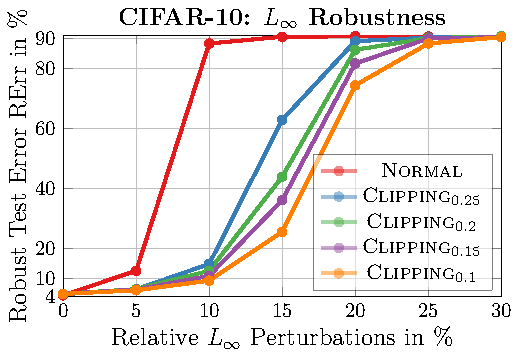
\includegraphics[width=0.4\textwidth]{c10_clipping_linf.pdf}
	\vspace*{-8px}
	\caption{\textbf{Weight Clipping Improves $L_\infty$ Robustness.} On \CifarT, we plot \RTE for \emph{relative} $L_\infty$ perturbations on weights: Random noise with $L_\infty$-norm smaller than or equal to $x\%$ of the weight range is applied. \Clipping clearly improves robustness. Again, the relative magnitude of noise is not affected by weight clipping. Note that $L_\infty$ noise usually affects all weights, while random bit errors affect only a portion of the weights.}
	\label{fig:supp-clipping-inf}
	\vspace*{-0.2cm}
\end{figure}

\figref{fig:supp-errors} splits the bit error distributions of \figref{fig:errors} into a $0$-to-$1$ flip and a $1$-to-$0$ bit flip map. The obtained maps, $p_{\text{1t0}}$ and $p_{\text{0t1}}$, contain per-bit flip probabilities for $1$-to-$0$ and $0$-to-$1$ bit flips at a given low voltage. In this particular profiled chip, \figref{fig:supp-errors} (bottom), $0$-to-$1$ flips are more likely. Similarly, \figref{fig:supp-errors} (right) shows that most  $0$-to-$1$ flips are actually persistent across time at that voltage \ie, not random transient errors. 
The following table summarizing the key statistics of the profiled chips: the overall bit error rate $p$, the rate of $1$-to-$0$ and $0$-to-$1$ flips $p_{\text{1t0}}$ and $p_{\text{0t1}}$, and the rate of persistent errors $p_{\text{sa}}$, all in \% at a specific supply voltage:

\begin{center}\small
\begin{tabular}{| l | c | c | c | c |}
	\hline
	Chip & $p$ & $p_{\text{0t1}}$ & $p_{\text{1t0}}$ & $p_{\text{sa}}$ \\
	\hline
	\multirow{2}{*}{1} & 2.744 & 1.27 & 1.47 & 1.223\\
	& 0.866 & 0.38 & 0.49 & 0.393\\
	\hline
	\multirow{3}{*}{2} & 4.707 &  3.443 & 1.091 & 0.627\\
	& 1.01 &  0.82 & 0.19 & 0.105\\
	& 0.136 & 0.115 & 0.021 & 0.01 \\
	\hline
	\multirow{2}{*}{3} & 2.297 & 1.81 & 0.48 & 0.204 \\
	& 0.597 & 0.496 & 0.0995 & 0.206 \\
	\hline
\end{tabular}
\end{center}

\begin{table*}[t]
	\centering
	\small
	\caption{\textbf{Impact of Quantization Scheme on Robustness.} Complementary to \tabref{tab:quantization-robustness}, we report \TE and \RTE for various bit error rates $p$ for the quantization scheme in \eqnref{eq:quantization} with global, per-layer and asymmetric quantization, $m = 8$ bits. Instead of quantizing into signed integer, using unsigned integers works better for asymmetric quantization. Furthermore, proper rounding instead of integer conversion also improves robustness. Note that influence on clean \TE is neglegible, \ie, the DNN can ``learn around'' these difference in quantization-aware training. Especially for $m = 4$ bit, the latter makes a significant difference in terms of robustness.}
	\label{tab:supp-quantization}
	\vspace*{-0.25cm}
	\begin{tabular}{| c | l | c | c | c | c | c | c | c |}
		\hline
		\multicolumn{9}{|c|}{\bfseries \CifarT: quantization robustness}\\
		\hline
		& Model & \multirow{2}{*}{\begin{tabular}{c}\TE\\in \%\end{tabular}} & \multicolumn{6}{c|}{\RTE in \%, $p$ in \% p=0.01}\\
		\cline{4-9}
		& (see text) && $0.01$ & $0.05$ & $0.1$ & $0.5$ & $1$ & $1.5$\\
		\hline
		\hline
		\multirow{5}{*}{\rotatebox{90}{$m = 8$ bit}} & \eqnref{eq:quantization}, global & 4.63 & 10.70 {\color{gray}\scriptsize ${\pm}$1.37} & 86.01 {\color{gray}\scriptsize ${\pm}$3.65} & 90.36 {\color{gray}\scriptsize ${\pm}$0.66} & 90.71 {\color{gray}\scriptsize ${\pm}$0.49} & 90.57 {\color{gray}\scriptsize ${\pm}$0.43} & --\\
		& \eqnref{eq:quantization}, per-layer (= \Normal) & 4.36 & 4.82 {\color{gray}\scriptsize ${\pm}$0.07} & 5.51 {\color{gray}\scriptsize ${\pm}$0.19} & 6.37 {\color{gray}\scriptsize ${\pm}$0.32} & 24.76 {\color{gray}\scriptsize ${\pm}$4.71} & 72.65 {\color{gray}\scriptsize ${\pm}$6.35} & 87.40 {\color{gray}\scriptsize ${\pm}$2.47}\\
		& +asymmetric & 4.36 & 5.76 {\color{gray}\scriptsize ${\pm}$0.09} & 6.47 {\color{gray}\scriptsize ${\pm}$0.22} & 7.85 {\color{gray}\scriptsize ${\pm}$0.46} & 40.78 {\color{gray}\scriptsize ${\pm}$7.56} & 76.72 {\color{gray}\scriptsize ${\pm}$7.01} & 85.83 {\color{gray}\scriptsize ${\pm}$2.58}\\
		& +unsigned & 4.42 & 6.58 {\color{gray}\scriptsize ${\pm}$0.13} & 6.97 {\color{gray}\scriptsize ${\pm}$0.28} & 7.49 {\color{gray}\scriptsize ${\pm}$0.41} & 17.00 {\color{gray}\scriptsize ${\pm}$2.77} & 54.57 {\color{gray}\scriptsize ${\pm}$8.58} & 83.18 {\color{gray}\scriptsize ${\pm}$3.94}\\
		& +rounded (= \Quant) & 4.32 & 4.60 {\color{gray}\scriptsize ${\pm}$0.08} & 5.10 {\color{gray}\scriptsize ${\pm}$0.13} & 5.54 {\color{gray}\scriptsize ${\pm}$0.2} & 11.28 {\color{gray}\scriptsize ${\pm}$1.47} & 32.05 {\color{gray}\scriptsize ${\pm}$6} & 68.65 {\color{gray}\scriptsize ${\pm}$9.23}\\
		\hline
		\hline
		\multirow{2}{*}{\rotatebox{90}{$4$ bit}} & integer conversion & 5.81 & 90.46 {\color{gray}\scriptsize ${\pm}$0.2} & 90.40 {\color{gray}\scriptsize ${\pm}$0.21} & 90.39 {\color{gray}\scriptsize ${\pm}$0.22} & 90.36 {\color{gray}\scriptsize ${\pm}$0.2} & 90.36 {\color{gray}\scriptsize ${\pm}$0.22} & 90.39 {\color{gray}\scriptsize ${\pm}$0.22}\\
		& proper rounding & 5.29 & 5.49 {\color{gray}\scriptsize ${\pm}$0.04} & 5.75 {\color{gray}\scriptsize ${\pm}$0.06} & 5.99 {\color{gray}\scriptsize ${\pm}$0.09} & 7.71 {\color{gray}\scriptsize ${\pm}$0.36} & 10.62 {\color{gray}\scriptsize ${\pm}$1.08} & 15.79 {\color{gray}\scriptsize ${\pm}$2.54}\\
		\hline
	\end{tabular}
	\vspace*{-0.1cm} 
\end{table*}

For evaluation, we assume that the DNN weights are mapped linearly onto the memory of these chips. The bit error maps are of size $8192 \times 128$ bits for chips 2 and 3 and $2048 \times 128$ bits for chip 1. Furthermore, to simulate various different mappings, we repeat this procedure with various offsets and compute average \RTE across all mappings. For results, we refer to \appref{subsec:supp-randbet-baselines}.

\subsection{Bounding Generalization to Random Bit Errors}
\label{subsec:supp-bound}

Let $w$ denote the final weights of a trained DNN $f$. We test $f$ using $n$ i.i.d. test examples, \ie, $(x_i,y_i)_{i=1}^n$. We denote by $w'$ the weights where each bit of $w$ is flipped with probability $p$ uniformly at random, corresponding to the error model from \secref{sec:errors}.
The expected \emph{clean} error  of $f$ is given by
\begin{align*}
	\Exp[\Id_{f(x;w)\neq y}] = \Pr(f(x;w)\neq y).
\end{align*}
The expected \emph{robust} error (regarding i.i.d. test examples drawn from the data distribution) with random bit errors in the (quantized) weights is
\begin{align*}
	\Exp[ \Id_{f(x;w')\neq y}] = \Pr( f(x;w')\neq y).
\end{align*}
Here, the weights of the neural network are themselves random variables. Therefore, with $x, y, w$, and $w'$ we denote the random variables corresponding to test example, test label, weights and weights bit random bit errors. With $x_j, y_j, w_i$ and $w'_i$ we denote actual examples. Then, the following proposition derives a simple, probabilistic bound on the deviation of expected robust error from the empirically measured one (\ie, \RTE in our experiments):

\begin{table*}[t]
	\centering
	\small
	\caption{\textbf{Weight Clipping Improves Robustness.} We report \TE and \RTE for various experiments on the robustness of weight clipping with $\wmax$, \ie, \Clipping[$\wmax$]. First, we show that the robustness benefit of \Clipping is independent of quantization-aware training, robustness also improves when applying post-training quantization. Then, we show results for both symmetric and asymmetric quantization. For the latter we demonstrate that label smoothing \cite{SzegedyCVPR2016} reduces the obtained robustness. This supports our hypothesis that weight clipping, driven by minimizing cross-entropy loss during training, improves robustness through redundancy.}
	\label{tab:supp-clipping}
	\vspace*{-0.25cm}
	\begin{tabular}{| c | l | c | c | c | c | c | c | c |}
		\hline
		\multicolumn{9}{|c|}{\bfseries \CifarT ($\mathbf{m = 8}$ bit): clipping robustness for post- and during-training quantization}\\
		\hline
		&Model & \multirow{2}{*}{\begin{tabular}{c}\TE\\in \%\end{tabular}} & \multicolumn{6}{c|}{\RTE in \%, $p$ in \% p=0.01}\\
		\cline{4-9}
		&&& $0.01$ & $0.05$ & $0.1$ & $0.5$ & $1$ & $1.5$\\
		\hline
		\hline
		\multirow{6}{*}{\rotatebox{90}{\begin{tabular}{@{}c@{}}Post-Training\\Asymmetric\end{tabular}}} & \Normal & 4.37 & 4.95 {\color{gray}\scriptsize ${\pm}$0.11} & 5.47 {\color{gray}\scriptsize ${\pm}$0.17} & 6.03 {\color{gray}\scriptsize ${\pm}$0.22} & 15.42 {\color{gray}\scriptsize ${\pm}$3.4} & 51.83 {\color{gray}\scriptsize ${\pm}$9.92} & 81.74 {\color{gray}\scriptsize ${\pm}$5.14}\\
		& \Quant & 4.27 & 4.59 {\color{gray}\scriptsize ${\pm}$0.08} & 5.10 {\color{gray}\scriptsize ${\pm}$0.13} & 5.54 {\color{gray}\scriptsize ${\pm}$0.15} & 10.59 {\color{gray}\scriptsize ${\pm}$1.11} & 30.58 {\color{gray}\scriptsize ${\pm}$6.05} & 63.72 {\color{gray}\scriptsize ${\pm}$6.89}\\
		& \Clipping[$0.25$] & 4.96 & 5.24 {\color{gray}\scriptsize ${\pm}$0.07} & 5.73 {\color{gray}\scriptsize ${\pm}$0.14} & 6.16 {\color{gray}\scriptsize ${\pm}$0.21} & 10.51 {\color{gray}\scriptsize ${\pm}$0.91} & 26.27 {\color{gray}\scriptsize ${\pm}$5.65} & 61.49 {\color{gray}\scriptsize ${\pm}$9.03}\\
		& \Clipping[$0.2$] & 5.24 & 5.48 {\color{gray}\scriptsize ${\pm}$0.05} & 5.87 {\color{gray}\scriptsize ${\pm}$0.09} & 6.23 {\color{gray}\scriptsize ${\pm}$0.13} & 9.47 {\color{gray}\scriptsize ${\pm}$0.7} & 19.78 {\color{gray}\scriptsize ${\pm}$3.58} & 43.64 {\color{gray}\scriptsize ${\pm}$8.2}\\
		& \Clipping[$0.15$] & 5.38 & 5.63 {\color{gray}\scriptsize ${\pm}$0.05} & 6.03 {\color{gray}\scriptsize ${\pm}$0.09} & 6.38 {\color{gray}\scriptsize ${\pm}$0.13} & 8.80 {\color{gray}\scriptsize ${\pm}$0.41} & 15.74 {\color{gray}\scriptsize ${\pm}$2.24} & 36.29 {\color{gray}\scriptsize ${\pm}$7.34}\\
		& \Clipping[$0.1$] & 5.32 & 5.52 {\color{gray}\scriptsize ${\pm}$0.04} & 5.82 {\color{gray}\scriptsize ${\pm}$0.06} & 6.05 {\color{gray}\scriptsize ${\pm}$0.07} & 7.45 {\color{gray}\scriptsize ${\pm}$0.26} & 9.80 {\color{gray}\scriptsize ${\pm}$0.62} & 17.56 {\color{gray}\scriptsize ${\pm}$3.08}\\
		\hline
		\hline
		\multirow{7}{*}{\rotatebox{90}{\begin{tabular}{@{}c@{}}Symmetric\\(during training)\end{tabular}}} & \Normal & 4.36 & 4.82 {\color{gray}\scriptsize ${\pm}$0.07} & 5.51 {\color{gray}\scriptsize ${\pm}$0.19} & 6.37 {\color{gray}\scriptsize ${\pm}$0.32} & 24.76 {\color{gray}\scriptsize ${\pm}$4.71} & 72.65 {\color{gray}\scriptsize ${\pm}$6.35} & 87.40 {\color{gray}\scriptsize ${\pm}$2.47}\\
		& \Quant & 4.39 & 4.77 {\color{gray}\scriptsize ${\pm}$0.08} & 5.43 {\color{gray}\scriptsize ${\pm}$0.21} & 6.10 {\color{gray}\scriptsize ${\pm}$0.32} & 17.11 {\color{gray}\scriptsize ${\pm}$3.07} & 55.35 {\color{gray}\scriptsize ${\pm}$9.4} & 82.84 {\color{gray}\scriptsize ${\pm}$4.52}\\
		& \Clipping[$0.25$] & 4.63 & 4.99 {\color{gray}\scriptsize ${\pm}$0.07} & 5.53 {\color{gray}\scriptsize ${\pm}$0.1} & 6.06 {\color{gray}\scriptsize ${\pm}$0.16} & 13.55 {\color{gray}\scriptsize ${\pm}$1.42} & 41.64 {\color{gray}\scriptsize ${\pm}$7.35} & 73.39 {\color{gray}\scriptsize ${\pm}$7.15}\\
		& \Clipping[$0.2$] & 4.50 & 4.79 {\color{gray}\scriptsize ${\pm}$0.06} & 5.25 {\color{gray}\scriptsize ${\pm}$0.09} & 5.65 {\color{gray}\scriptsize ${\pm}$0.16} & 9.64 {\color{gray}\scriptsize ${\pm}$0.99} & 21.37 {\color{gray}\scriptsize ${\pm}$4.23} & 45.68 {\color{gray}\scriptsize ${\pm}$7.9}\\
		& \Clipping[$0.15$] & 5.18 & 5.42 {\color{gray}\scriptsize ${\pm}$0.05} & 5.76 {\color{gray}\scriptsize ${\pm}$0.08} & 6.07 {\color{gray}\scriptsize ${\pm}$0.09} & 8.36 {\color{gray}\scriptsize ${\pm}$0.43} & 13.80 {\color{gray}\scriptsize ${\pm}$1.45} & 24.70 {\color{gray}\scriptsize ${\pm}$3.77}\\
		& \Clipping[$0.1$] & 4.86 & 5.07 {\color{gray}\scriptsize ${\pm}$0.04} & 5.34 {\color{gray}\scriptsize ${\pm}$0.06} & 5.59 {\color{gray}\scriptsize ${\pm}$0.1} & 7.12 {\color{gray}\scriptsize ${\pm}$0.3} & 9.44 {\color{gray}\scriptsize ${\pm}$0.7} & 13.14 {\color{gray}\scriptsize ${\pm}$1.79}\\
		& \Clipping[$0.05$] & 5.56 & 5.70 {\color{gray}\scriptsize ${\pm}$0.03} & 5.89 {\color{gray}\scriptsize ${\pm}$0.06} & 6.03 {\color{gray}\scriptsize ${\pm}$0.08} & 6.68 {\color{gray}\scriptsize ${\pm}$0.14} & 7.31 {\color{gray}\scriptsize ${\pm}$0.2} & 8.06 {\color{gray}\scriptsize ${\pm}$0.36}\\
		\hline
		\hline
		\multirow{11}{*}{\rotatebox{90}{\begin{tabular}{@{}c@{}}{\color{red}\textbf{A}}symmetric (default) quant.\\(during training)\end{tabular}}} & \Normal & 4.36 & 4.82 {\color{gray}\scriptsize ${\pm}$0.07} & 5.51 {\color{gray}\scriptsize ${\pm}$0.19} & 6.37 {\color{gray}\scriptsize ${\pm}$0.32} & 24.76 {\color{gray}\scriptsize ${\pm}$4.71} & 72.65 {\color{gray}\scriptsize ${\pm}$6.35} & 87.40 {\color{gray}\scriptsize ${\pm}$2.47}\\
		& \Quant & 4.32 & 4.60 {\color{gray}\scriptsize ${\pm}$0.08} & 5.10 {\color{gray}\scriptsize ${\pm}$0.13} & 5.54 {\color{gray}\scriptsize ${\pm}$0.2} & 11.28 {\color{gray}\scriptsize ${\pm}$1.47} & 32.05 {\color{gray}\scriptsize ${\pm}$6} & 68.65 {\color{gray}\scriptsize ${\pm}$9.23}\\
		& \Clipping[$0.25$] & 4.58 & 4.84 {\color{gray}\scriptsize ${\pm}$0.05} & 5.29 {\color{gray}\scriptsize ${\pm}$0.12} & 5.71 {\color{gray}\scriptsize ${\pm}$0.16} & 10.52 {\color{gray}\scriptsize ${\pm}$1.14} & 27.95 {\color{gray}\scriptsize ${\pm}$4.16} & 62.46 {\color{gray}\scriptsize ${\pm}$8.89}\\
		& \Clipping[$0.2$] & 4.63 & 4.91 {\color{gray}\scriptsize ${\pm}$0.05} & 5.28 {\color{gray}\scriptsize ${\pm}$0.08} & 5.62 {\color{gray}\scriptsize ${\pm}$0.11} & 8.27 {\color{gray}\scriptsize ${\pm}$0.35} & 18.00 {\color{gray}\scriptsize ${\pm}$2.84} & 53.74 {\color{gray}\scriptsize ${\pm}$8.89}\\
		& \Clipping[$0.15$] & 4.42 & 4.66 {\color{gray}\scriptsize ${\pm}$0.05} & 5.01 {\color{gray}\scriptsize ${\pm}$0.09} & 5.31 {\color{gray}\scriptsize ${\pm}$0.12} & 7.81 {\color{gray}\scriptsize ${\pm}$0.6} & 13.08 {\color{gray}\scriptsize ${\pm}$2.21} & 23.85 {\color{gray}\scriptsize ${\pm}$5.07}\\
		& \Clipping[$0.1$] & 4.82 & 5.04 {\color{gray}\scriptsize ${\pm}$0.04} & 5.33 {\color{gray}\scriptsize ${\pm}$0.07} & 5.58 {\color{gray}\scriptsize ${\pm}$0.1} & 6.95 {\color{gray}\scriptsize ${\pm}$0.24} & 8.93 {\color{gray}\scriptsize ${\pm}$0.46} & 12.22 {\color{gray}\scriptsize ${\pm}$1.29}\\
		& \Clipping[$0.05$] & 5.44 & 5.59 {\color{gray}\scriptsize ${\pm}$0.04} & 5.76 {\color{gray}\scriptsize ${\pm}$0.07} & 5.90 {\color{gray}\scriptsize ${\pm}$0.07} & 6.53 {\color{gray}\scriptsize ${\pm}$0.13} & 7.18 {\color{gray}\scriptsize ${\pm}$0.16} & 7.92 {\color{gray}\scriptsize ${\pm}$0.25}\\
		\cline{2-9} 
		& \Clipping[$0.2$]+LS & 4.48 & 4.77 {\color{gray}\scriptsize ${\pm}$0.05} & 5.19 {\color{gray}\scriptsize ${\pm}$0.1} & 5.55 {\color{gray}\scriptsize ${\pm}$0.12} & 9.46 {\color{gray}\scriptsize ${\pm}$0.82} & 32.49 {\color{gray}\scriptsize ${\pm}$5.07} & 68.60 {\color{gray}\scriptsize ${\pm}$7.33}\\
		& \Clipping[$0.15$]+LS & 4.67 & 4.86 {\color{gray}\scriptsize ${\pm}$0.05} & 5.23 {\color{gray}\scriptsize ${\pm}$0.08} & 5.83 {\color{gray}\scriptsize ${\pm}$0.12} & 7.99 {\color{gray}\scriptsize ${\pm}$0.43} & 29.40 {\color{gray}\scriptsize ${\pm}$6.99} & 68.99 {\color{gray}\scriptsize ${\pm}$8.48}\\
		& \Clipping[$0.1$]+LS & 4.82 & 5.05 {\color{gray}\scriptsize ${\pm}$0.04} & 5.37 {\color{gray}\scriptsize ${\pm}$0.08} & 6.10 {\color{gray}\scriptsize ${\pm}$0.11} & 7.36 {\color{gray}\scriptsize ${\pm}$0.4} & 10.59 {\color{gray}\scriptsize ${\pm}$1.01} & 18.31 {\color{gray}\scriptsize ${\pm}$2.84}\\
		& \Clipping[$0.05$]+LS & 5.30 & 5.43 {\color{gray}\scriptsize ${\pm}$0.03} & 5.63 {\color{gray}\scriptsize ${\pm}$0.06} & 6.43 {\color{gray}\scriptsize ${\pm}$0.07} & 6.51 {\color{gray}\scriptsize ${\pm}$0.15} & 7.30 {\color{gray}\scriptsize ${\pm}$0.23} & 8.06 {\color{gray}\scriptsize ${\pm}$0.38}\\
		\hline
	\end{tabular}
	\vspace*{-0.1cm}
\end{table*}

\begin{proposition}
	\label{prop:bound}
	Let $w'_i$, $i = 1,\ldots,l$ be $l$ examples of weights bit random bit errors (each bit flipped with probability $p$). Then it holds
	\begin{align*}
		\Pr\Big( \frac{1}{nl}&\sum_{j=1}^n \sum_{i=1}^l \Id_{f(x_j;w'_i)\neq y_j} - \Pr(f(x;w')\neq y)\geq \epsilon\Big)\\
		&\quad\leq (n+1) e^{-n\epsilon^2 \frac{l}{(\sqrt{l}+\sqrt{n})^2}}.
	\end{align*}
	As alternative formulation, with probability $1-\delta$ it holds
	\begin{align*}
		\Pr( f(x; w'_i)\neq y) < & \frac{1}{nl}\sum_{j=1}^n \sum_{i=1}^l \Id_{f(x_j; w'_i)\neq y_j}\\ &+ \quad \leq\sqrt{\frac{\log\Big(\frac{n+1}{\delta}\Big)}{n}} \frac{\sqrt{l}+\sqrt{n}}{\sqrt{l}}.
	\end{align*} 
\end{proposition}
{\small
\begin{proof}
Let $0<\alpha<1$. Using the Hoeffding inequality and union bound, we have:
\begin{align*}
	&\Pr\Big(\maxop_{j=1,\ldots,n} \frac{1}{l}\sum_{i=1}^l \Id_{f(x_j; w'_i)\neq y_j} - \Exp_{w'}[\Id_{f(x_j; w')\neq y_j}] > \alpha\epsilon\Big) \\
	=& \Pr\Big(\bigcup_{j=1,\ldots,n}\big\{ \frac{1}{l}\sum_{i=1}^l \Id_{f(x_j; w'_i)\neq y_j} - \Exp_{w'}[\Id_{f(x_j; w')\neq y_j}] > \alpha\epsilon\big\}\Big)\\
	&\leq \; n\, e^{-l\alpha^2 \epsilon^2}.
\end{align*}
Then, again by Hoeffding's inequality, it holds:
\begin{align*}
	&\Pr\Big( \frac{1}{n}\sum_{j=1}^n \Exp_{w'}[\Id_{f(x_j; w')\neq y_j}]
	- \Exp_{x,y}[\Exp_{w'}[\Id_{f(x; w')\neq y}]] > (1-\alpha) \epsilon \Big)\\
	&\leq \; e^{-n\epsilon^2 (1-\alpha)^2}.
\end{align*}
Thus, using
\begin{align*}
	a + b>\epsilon \Longrightarrow \{a > \alpha \epsilon\} \cup \{b > (1-\alpha)\epsilon\}
\end{align*}
gives us:
\begin{align*}
	&\Pr\Big( \frac{1}{nl}\sum_{j=1}^n \sum_{i=1}^l \Id_{f(x_j; w'_i)\neq y_j} - \Pr( f(x; w')\neq y)\geq \epsilon\Big)\\
	=& \Pr\Big( \frac{1}{n}\sum_{j=1}^n \big(\frac{1}{l}\sum_{i=1}^l \Id_{f_{w'_i}(x_j)\neq y_j} - \Exp_{w'}[\Id_{f(x_j; w'_i)\neq y_j}]\big)\\
	 +& \frac{1}{n}\sum_{j=1}^n \Exp_{w'}[\Id_{f(x_j; w'_i)\neq y_j}] - \Pr( f(x; w')\neq y)\geq \epsilon\Big)\\
	\leq & \Pr\Big( \frac{1}{n}\sum_{j=1}^n \big(\frac{1}{l}\sum_{i=1}^l \Id_{f(x_j; w'_i)\neq y_j} - \Exp_{w'}[\Id_{f(x_j; w')\neq y_j}]\big)>\alpha \epsilon\Big)\\
	+& \Pr\Big( \frac{1}{n}\sum_{j=1}^n \Exp_{w'}[\Id_{f(x_j; w')\neq y_j}] - \Pr( f(x; w')\neq y)\geq (1-\alpha)\epsilon\Big)\\
	\leq &  n\, e^{-l\alpha^2 \epsilon^2} + e^{-n\epsilon^2 (1-\alpha)^2} 
\end{align*}
Having both exponential terms have the same exponent yields $\alpha=\frac{\sqrt{n}}{\sqrt{l}+\sqrt{n}}$ and we get the upper bound of the proposition.
\end{proof}
}

\textbf{Remarks:}
The samples of bit error injected weights $\{w'_i\}_{i=1}^l$ can actually be different for any test example $(x_j, y_j)$, even though this is not the case in our evaluation. Thus, the above bound involves a stronger result: for any test example, the empirical test error with random bit errors (\ie, robust test error \RTE) and the expected one have to be similar with the same margin. Note also that this bound holds for any fixed bit error distribution as the only requirement is that the bit error patterns we draw are i.i.d. but not the bit errors on the pattern.
In \appref{subsec:experiments-stress}, we consider results with $l = 10^6$, \ie, $l \gg n$ with $n = 10^4$ on \CifarT such that $\nicefrac{l}{(\sqrt{l}+\sqrt{n})^2}$ tends towards one. With $\delta=0.99$ the excess term $\sqrt{\frac{\log\Big(\frac{n+1}{\delta}\Big)}{n}} \frac{\sqrt{l}+\sqrt{n}}{\sqrt{l}}$ in the Proposition is equal to $4.1\%$. Thus larger test sets would be required to get stronger guarantees e.g. for $n=10^5$ one would get $1.7\%$.

\section{Quantization and Bit Manipulation in PyTorch}
\label{sec:supp-implementation}

Our fixed-point quantization $Q$ in \eqnref{eq:quantization} quantizes weights $w_i \in [-\qmax, \qmax] \subset \mathbb{R}$ into signed integers $\{-2^{m-1}-1,\ldots,2^{m-1}-1\}$. Here, the quantization range $[-\qmax,\qmax]$ is symmetric around zero. Note that zero is represented exactly. To implement asymmetric quantization, as outlined in \secref{subsec:robustness-quantization}, the same scheme can be used to quantize weights $w_i \in [\qmin, \qmax]$ within any arbitrary, potentially asymmetric, interval. To this end, \eqnref{eq:quantization} with $\qmax = 1$ is used and the weights in $[\qmin,\qmax]$ are mapped linearly to $[-1, 1]$ using the transformation $N$:
\begin{align}
	N(w_i) = \left(\frac{w_i - \qmin}{\qmax - \qmin}\right)\cdot 2 - 1.\label{eq:asymmetric-quantization}
\end{align}
Generally, $\qmin$ and $\qmax$ are chosen to reflect minimum and maximum weight value -- either from all weights (global quantization) or per-layer.
Furthermore, we argue that asymmetric quantization becomes more robust when using \emph{unsigned} integers as representation. In this case, \eqnref{eq:quantization} can be adapted using a simple additive term:
\begin{align}
	\begin{split}
		Q(w_i) &= \left\lceil \frac{w_i}{\Delta}\right\rfloor + (2^{m - 1} - 1)\\
		Q^{-1}(v_i) &= \Delta (v_i - (2^{m - 1} - 1))
	\end{split}\label{eq:unsigned-quantization}
\end{align}
We use asymmetric quantization using $N$ in \eqnref{eq:asymmetric-quantization} with \eqnref{eq:unsigned-quantization} as our \emph{robust} fixed-point quantization.

\begin{table}[t]
	\centering
	\small
	\caption{\textbf{Batch Normalization not Robust.} \RTE with group normalization (GN) or batch normalization (BN). \RTE increases when using BN even though clean \TE improves slightly compared GN. However, using batch statistics at test time (\ie, ``training mode'' in PyTorch) improves \RTE significantly indicating that the statistics accumulated throughout training do not account for random bit errors. We use \textbf{group normalization as default.}}
	\label{tab:supp-bn}
	\vspace*{-0.25cm}
	\hspace*{-0.25cm}
	\begin{tabular}{| c | l | c | c | c |}
		\hline
		\multicolumn{5}{|c|}{\bfseries \CifarT ($\mathbf{m = 8}$ bit): robustness of BN}\\
		\hline
		&& \multirow{2}{*}{\begin{tabular}{@{}c@{}}\TE\\in \%\end{tabular}} & \multicolumn{2}{c|}{\RTE in \%}\\
		\hline
		&& & $p{=}0.1$ & $p{=}0.5$\\
		\hline
		\hline
		\multirow{2}{*}{GN} & \Normal & 4.32 & 5.54 & 11.28\\
		& \Clipping[$0.1$] & 4.82 & 5.58 & 6.95\\
		\hline
		\hline
		\multicolumn{5}{|c|}{\textbf{BN w/ \emph{Accumulated} Statistics}}\\
		\hline
		\multirow{2}{*}{BN} & \Normal & 3.83 & 6.36 & 52.52\\
		& \Clipping[$0.1$] & 4.46 & 5.32 & 8.25\\
		\hline
		\hline
		\multicolumn{5}{|c|}{\textbf{BN w/ Batch Statistics at Test Time}}\\
		\hline
		\multirow{2}{*}{BN} & \Normal & 3.83 & 6.65 & 9.63\\
		& \Clipping[$0.1$] & 4.46 & 6.57 & 7.29\\
		\hline
	\end{tabular}
	\vspace*{-0.1cm}
\end{table}

Following \secref{subsec:robustness-quantization}, we implement ``fake'' fixed-point quantization for quantization-aware training and bit error injection directly in PyTorch \cite{PaszkeNIPSWORK2017}. Here, fake quantization means that computation is performed in floating point, but before doing a forward pass, the DNN is quantized and dequantized, \ie, $w_q = Q^{-1}(Q(w))$ in \algref{alg:training}. Note that we quantize into \emph{unsigned} $8$ bit integers, irrespective of the target precision $m \leq 8$. To later induce random bit errors, the $8 - m$ most significant bits (MSBs) are masked for $m < 8$. Bit manipulation of unsigned $8$ bit integers is then implemented in C/CUDA and interfaced to Python using CuPy \cite{cupy} or CFFI \cite{cffi}. These functions can directly operate on PyTorch tensors, allowing bit manipulation on the CPU as well as the GPU. We will make our code publicly available to faciliate research into DNN robustness against random bit errors.

\section{Weight Clipping with Group/Batch Normalization}
\label{sec:supp-clipping}

While weight clipping, \ie, globally constraining weights to $[-\wmax, \wmax]$ during training, is easy to implement, we make a simple adjustment to group and batch normalization layers: we reparameterize the scale parameter $\alpha$ of batch/group normalization, which usually defaults to $\alpha = 1$ and may cause problems when clipped, \eg, to $[-0.1, 0.1]$. In particular with aggressive weight clipping, $\alpha \leq \wmax < 1$, the normalization layers loose their ability to represent the identity function, considered important for batch normalization in \cite{IoffeICML2015}. Our reparameterization introduces a learnable, auxiliary parameter $\alpha'$ such that $\alpha$ as $\alpha = 1 + \alpha'$ to solve this problem.